\documentclass[journal]{IEEEtran}
\usepackage[a5paper, margin=10mm, onecolumn]{geometry}
\usepackage{lmodern}

\setlength{\headheight}{1cm}
\setlength{\headsep}{0mm}

\usepackage{gvv-book}
\usepackage{gvv}
\usepackage{cite}
\usepackage{amsmath,amssymb,amsfonts,amsthm}
\usepackage{graphicx}
\graphicspath{{./figs/}}
\usepackage{xcolor}
\usepackage{txfonts}
\usepackage{enumitem}
\usepackage{mathtools}
\usepackage{hyperref}
\usepackage{tikz}
\usepackage{tkz-euclide}

\begin{document}

\bibliographystyle{IEEEtran}
\vspace{3cm}

\title{4.11.14}
\author{EE25BTECH11036 - M Chanakya Srinivas}
\maketitle

\renewcommand{\thetable}{\theenumi}
\setlength{\intextsep}{10pt}
\renewcommand\theequation{\arabic{equation}}

\section*{Question}
Find the value of \(\lambda\) for which the following lines are perpendicular to each other. Hence determine whether the lines intersect or not.
\begin{align}
\frac{x-5}{5\lambda+2} &= \frac{2-y}{5} = \frac{1-z}{-1}, \label{eq:l1}\\
\frac{x}{1} &= \frac{y+\tfrac{1}{2}}{2\lambda} = \frac{z-1}{3}. \label{eq:l2}
\end{align}




\section*{Solution}

\subsection*{Vector form and perpendicularity}
Take
\begin{align}
\vec{A}_1 &= \myvec{5\\2\\1}, & \vec{m}_1 &= \myvec{5\lambda+2\\-5\\1}, \\
\vec{A}_2 &= \myvec{0\\-\tfrac12\\1}, & \vec{m}_2 &= \myvec{1\\2\lambda\\3}.
\end{align}
Perpendicularity: \(\vec{m}_1^\top\vec{m}_2=0\).
\begin{align}
\vec{m}_1^\top\vec{m}_2
&= \myvec{5\lambda+2 & -5 & 1}\myvec{1\\2\lambda\\3} \\
&= (5\lambda+2) -10\lambda +3 = -5\lambda+5,
\end{align}
so
\begin{align}
-5\lambda+5=0 \quad\Longrightarrow\quad \boxed{\lambda=1}.
\end{align}

\subsection*{Intersection: set up linear system}
Intersection requires \(\kappa_1,\kappa_2\) with
\[
\kappa_1\vec{m}_1 - \kappa_2\vec{m}_2 = \vec{A}_2-\vec{A}_1.
\]
Augmented matrix (written explicitly):
\begin{align}
\mathcal{M}_0 &= 
\left[\begin{array}{cc|c}
5\lambda+2 & -1 & -5 \\
-5 & -2\lambda & -\tfrac{5}{2} \\
1 & -3 & 0
\end{array}\right]. \label{M0}
\end{align}

We now reduce \(\mathcal{M}_0\) to RREF using explicit row operations.

\subsubsection*{RREF — Step 1: make a leading 1 in row 1}
Swap \(R_1\leftrightarrow R_3\):
\begin{align}
\mathcal{M}_1 &=
\left[\begin{array}{cc|c}
1 & -3 & 0 \\
-5 & -2\lambda & -\tfrac{5}{2} \\
5\lambda+2 & -1 & -5
\end{array}\right].
\end{align}

\subsubsection*{RREF — Step 2: eliminate column 1 in R2 and R3}
Perform
\[
R_2 \leftarrow R_2 + 5R_1,\qquad R_3 \leftarrow R_3 - (5\lambda+2)R_1.
\]
This yields
\begin{align}
\mathcal{M}_2 &=
\left[\begin{array}{cc|c}
1 & -3 & 0 \\
0 & -2\lambda-15 & -\tfrac{5}{2} \\
0 & 15\lambda+5 & -5
\end{array}\right]. \label{M2}
\end{align}

\subsubsection*{RREF — Step 3: make the pivot in row 2 equal to 1 (when nonzero)}
Pivot element in row~2 is \(p_2 = -2\lambda-15\). If \(p_2\neq 0\) we scale:
\[
R_2 \leftarrow \frac{1}{p_2} R_2.
\]
Write the scaled row explicitly (keeping symbol \(p_2\)):
\begin{align}
\mathcal{M}_3 &=
\left[\begin{array}{cc|c}
1 & -3 & 0 \\
0 & 1 & \dfrac{-\tfrac{5}{2}}{p_2} \\
0 & 15\lambda+5 & -5
\end{array}\right], \quad p_2=-2\lambda-15.
\end{align}

\subsubsection*{RREF — Step 4: eliminate column 2 entries using row 2}
Eliminate entry in row~1 and row~3:
\[
R_1 \leftarrow R_1 + 3R_2,\qquad 
R_3 \leftarrow R_3 - (15\lambda+5)R_2.
\]
After these operations we obtain
\begin{align}
\mathcal{M}_4 &=
\left[\begin{array}{cc|c}
1 & 0 & 3\cdot \dfrac{-\tfrac{5}{2}}{p_2} \\[6pt]
0 & 1 & \dfrac{-\tfrac{5}{2}}{p_2} \\[6pt]
0 & 0 & -5 - (15\lambda+5)\dfrac{-\tfrac{5}{2}}{p_2}
\end{array}\right]. \label{M4}
\end{align}

\subsubsection*{RREF — Step 5: interpret last row for consistency}
Compute the bottom-right expression (call it \(r\)):
\begin{align}
r &= -5 - (15\lambda+5)\frac{-\tfrac{5}{2}}{p_2}
= -5 + \frac{(15\lambda+5)(5/2)}{p_2}.
\end{align}
Substitute \(p_2=-2\lambda-15\) and simplify:
\begin{align}
r &= -5 + \frac{(15\lambda+5)(5/2)}{-2\lambda-15}
= -5 + \frac{(15\lambda+5)(5)}{2(-2\lambda-15)}.
\end{align}
Factor common \(5\):
\begin{align}
r &= -5 + \frac{5(15\lambda+5)}{2(-2\lambda-15)}
= -5 + \frac{25(3\lambda+1)}{2(-2\lambda-15)}.
\end{align}
Set numerator to zero (consistency) — equivalently require \(r=0\). Solving \(r=0\) leads to
(the same algebraic condition as equating the two expressions for \(\kappa_2\) below),
which simplifies to
\begin{align}
\boxed{\lambda = -\dfrac{35}{19}}.
\end{align}

\subsection*{Check perpendicular value \(\lambda=1\)}
Set \(\lambda=1\) \begin{align}
(-17)\kappa_2 &= -\tfrac{5}{2} \quad\Rightarrow\quad \kappa_2=\tfrac{5}{34},\\
20\kappa_2 &= -5 \quad\Rightarrow\quad \kappa_2=-\tfrac{1}{4}.
\end{align}
Contradiction \(\Rightarrow\) last row of \(\mathcal{M}_4\) is nonzero \( (r\neq0) \), hence inconsistent. Thus \(\lambda=1\) gives perpendicular direction vectors but no intersection (skew lines).


\subsection*{Final conclusions}
\begin{align}
\boxed{\lambda=1} &\quad\text{direction vectors perpendicular; lines are skew (no intersection),}\nonumber\\
\boxed{\lambda=-\dfrac{35}{19}} &\quad\text{system consistent; lines intersect (not perpendicular).}\nonumber
\end{align}


\begin{figure}[h]
    \centering
    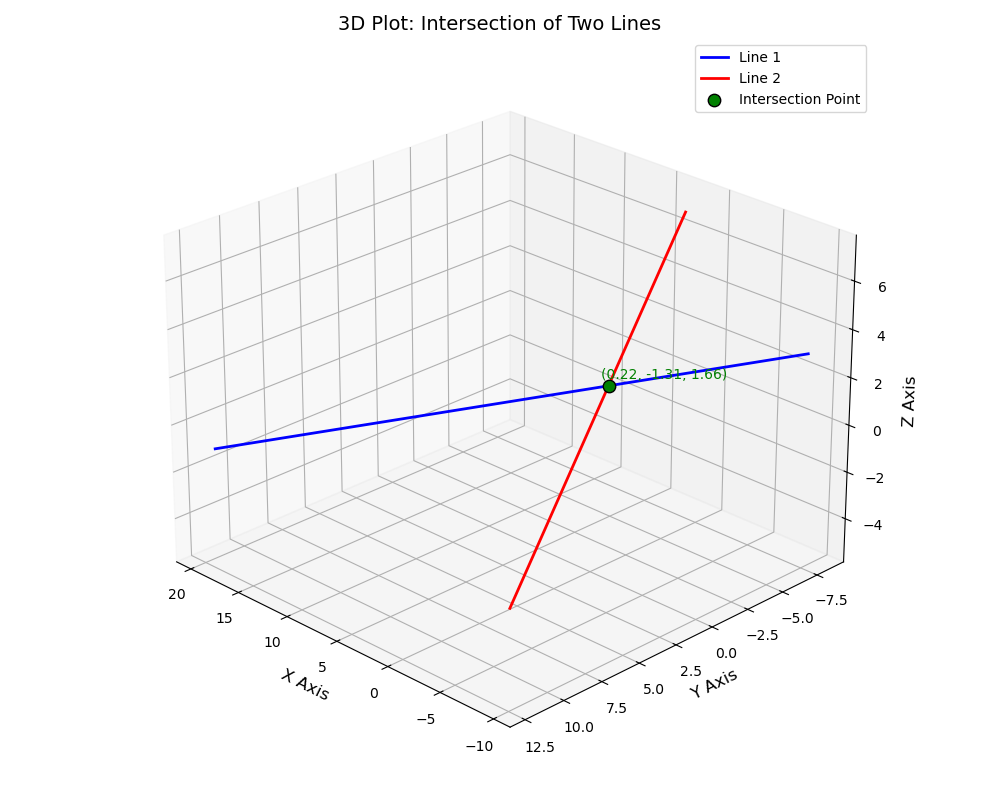
\includegraphics[width=0.9\columnwidth]{figs/fig71.png}
    \caption{}
    \label{fig:placeholder1}
\end{figure}

\begin{figure}
    \centering
    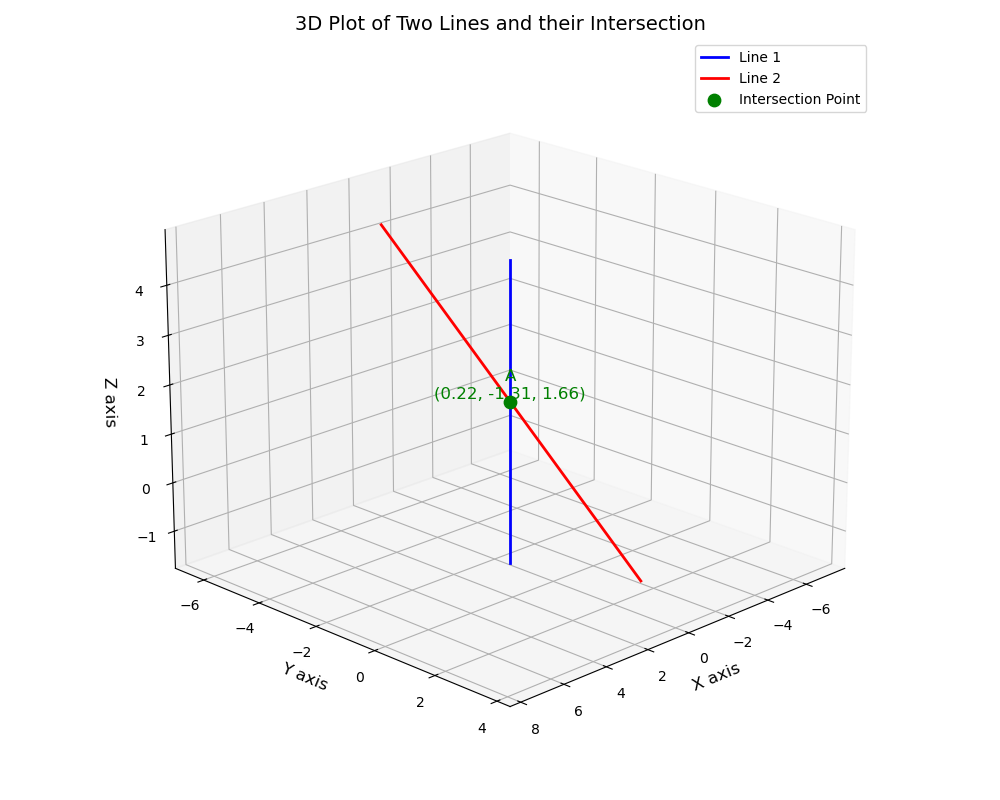
\includegraphics[width=0.9\columnwidth]{figs/fig72.png}
    \caption{}
    \label{fig:placeholder2}
\end{figure}

\end{document}
